\documentclass[11pt]{beamer}
%\usepackage[utf8]{luainputenc}
\usepackage{fontspec}

\usepackage[T1]{fontenc}
\usepackage{lmodern}
\usepackage[english]{babel}
\usepackage{amsmath}
\usepackage{amsfonts}
\usepackage{amssymb}
\usepackage{graphicx}
\usetheme{Madrid}

\setmainfont{Meiryo UI}
\newcommand{\colurl}[2][blue]{\textcolor{#1}{\underline{\url{#2}}\smallskip}}%

%\setmathfont{normal}

\begin{document}
	\author{Jonathan LEVY}
	\title{Research Project}
	\subtitle{Acceleration of non-rigid image registration with Tensor Cores}
	%\logo{}
	%\institute{}
	\date{\today}
	%\subject{}
	%\setbeamercovered{transparent}
	\setbeamertemplate{navigation symbols}{}
	\setbeamertemplate{caption}[numbered]
	
	
\begin{frame}[plain]
	\maketitle
\end{frame}

	\include{01-plan}
	\section{My cursus}
	
\begin{frame}{Cursus}
	\begin{columns}
		\column{0.45\textwidth}
		\begin{center}
			About me:
		\end{center}
			\begin{itemize}
				\item Jonathan LEVY
				\item MSc student in Embedded Systems, TU Delft (Netherlands)
				\item Multiple majors \& countries
			\end{itemize}
		\column{0.65\textwidth}

%		\begin{itemize}
%			\item \emph{Classe Préparatoire PTSI/PT*}
%			\item Ecole Normale Supérieure de Rennes (BSc, Master in Teaching)
%			\item \emph{Agrégation} in Engineering, CS track
%			\item MSc Embedded Systems, TU Delft
%		\end{itemize}
		\begin{figure}
			\centering
			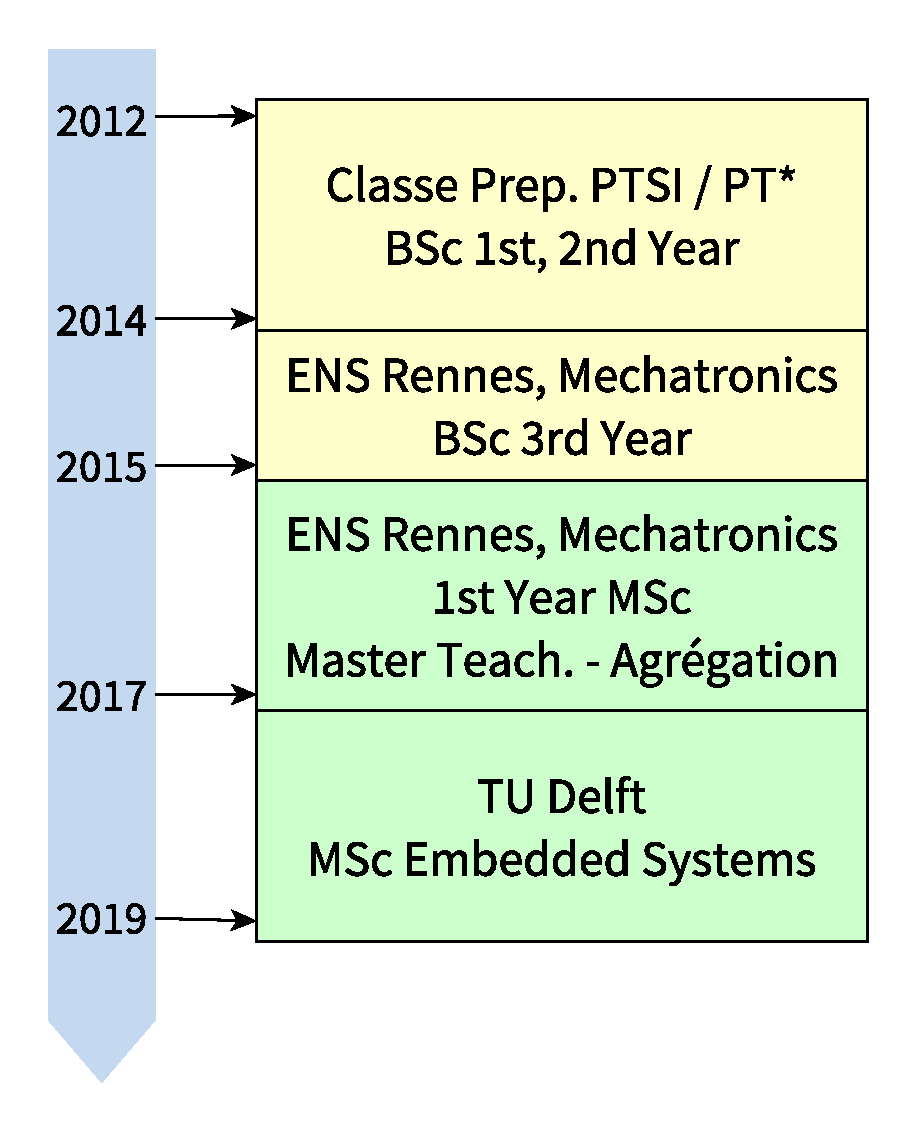
\includegraphics[width=0.7\linewidth]{timeline_studies}
		\end{figure}
	\end{columns}
\end{frame}
	
\begin{frame}{Current work}

	\begin{center}
		Since September 2019:
		
		GASAL2 : GPU-accelerated library for DNA alignment
	\end{center}
	\begin{columns}
		\column{0.02\textwidth}
		\column{0.9\textwidth}
		\begin{itemize}
			\item[When]	First as Extra Project, then MSc Thesis
			\item[Languages] C/C++ and CUDA
			\item[Algorithm] Smith-Waterman - optimal alignment for short pair
		\end{itemize}	
	\end{columns}

	\bigskip
	\textbf{Goal: integrate in the \emph{Burrough-Wheeler Aligner, "BWA"}}
	\bigskip
	
	\colurl{https://github.com/j-levy/GASAL2}
	\colurl{https://github.com/j-levy/bwa-gasal2} $\leftarrow$ private repository
	
\end{frame}
	
	\section{Research Project proposal}
	\begin{frame}{Research Proposal}
	\begin{center}
		\textbf{Acceleration of non-rigid image registration with Tensor Cores}
	\end{center}
	\begin{columns}
		\column{0.55\textwidth}
		\begin{itemize}
			\item Image registration: aligning 2 images
			\item \emph{Non-rigid}: various deformations allowed
			\item Use next-gen GPUs for acceleration
			\item \textbf{Goal: get closer to real-time (currently: seconds) for surgery} 
		\end{itemize}

		\column{0.45\textwidth}
		\begin{figure}
			\includegraphics[width=\textwidth]{registration}
			\caption[Deformations]{Different types of deformation.}
			\label{fig:registration}	
		\end{figure}

	\end{columns}
	
\end{frame}
	\begin{frame}{The Volta Architecture}
	
\end{frame}
	\begin{frame}{Tensor Cores}
	

		\begin{center}
			\begin{minipage}{0.5\textwidth}
				\centering
				\begin{itemize}
					\item[WHAT] Matrix-matrix multiplication
					\item[HOW] Mixed precision
					\item[WHY] Deep Learning
				\end{itemize}
			\end{minipage}

			\begin{figure}
				\includegraphics[width=\textwidth]{tensor_core_op}
				\caption{Operation done by a Tensor Core}
			\end{figure}
		\end{center}


	

\end{frame}
	\begin{frame}{Registration steps}
		% summarize steps

	
\end{frame}
	\begin{frame}{B-Splines model}
	\begin{center}
			\begin{minipage}{0.95\textwidth}
			\centering
			\begin{itemize}	
				\item[GOAL] Find optimal transformation $T: (x,y,z) \longmapsto (x', y', z')$
				\item[ALGO]	Spline-based Free-Form Deformation (FFD) : 3D deformation model	using net of points $\phi_{x,y,z}$
			\end{itemize}
		\end{minipage}
		\begin{equation}
	\mathnormal{
		T(x,y,z) = \newline
		\sum _{l=0}^{3}\sum _{m=0}^{3}\sum _{n=0}^{3}{B}_{l}\left(u\right){B}_{m}\left(v\right){B}_{n}\left(w\right){\phi }_{i+l,j+m,k+n}
	}
	\end{equation}
	
	\begin{columns}
		\column{0.4\textwidth}
			Tensor product $\implies$ Calculation by Tensor Cores possible
			
			Each point affects is 4 direct neighbours
		\column{0.6\textwidth}
		\begin{figure}
			\includegraphics[width=\textwidth]{control_net}
		\end{figure}
	\end{columns}
	
	

	
	\end{center}


	
\end{frame}
	\begin{frame}{Similarity score and Entropy}
	
	
%	\begin{columns}
%		\column{0.5\textwidth}
%			\begin{figure}
%				\includegraphics[width=0.5\textwidth]{joint_histogram}
%				\caption{\tiny Joint histogram calculation, from Groots \emph{et al.}, \emph{Practical Examples of GPU Computing Optimization Principles} (2010)}
%				\label{fig:joint_histogram}
%			\end{figure}
%		\column{0.5\textwidth}
%			Joint histogram: matrix $M$
%			$m_{i,j}$ = number of pixels at same position having values i (1st image) and j (second image)
%		Similar images $\implies$ fills diagonal
		
%		For each cell, calculate
%	\end{columns}
	
	$\mathnormal{C_{similarity}}$ relies on histograms and entropy calculation. 
	
	A formula for entropy $H(X)$:
	\begin{equation}
		\mathnormal{H\left(X\right)=-\sum _{i=1}^{n}{P}_{i} * log_{2}\left({P}_{i}\right)}
	\end{equation}
	with:
	\begin{itemize}
		\item $\mathnormal{n}$ the number of different values for pixels,
		\item $\mathnormal{P_{i}}$ probablity distribution of the value $i$ (values of histogram)
	\end{itemize}
	
	Sum of products : feasible with matrix-matrix multiplication
	
	$\implies$ Doable by Tensor cores.
	

\end{frame}
	\begin{frame}{Work proposal}
	Provide a library for accelerated calculation:
	
	\begin{enumerate}
		\item Accelerate entropy (NMI) with tensor cores
		
		\item Accelerated B-Splines using tensor cores too

		\item Quantify precision loss

		\item Send results for rendering (visual output)
	\end{enumerate}

	\hspace{0.035\textwidth} $\implies$ Generic functions
	
	\hspace{0.035\textwidth} $\implies$ Reusable
	
	\hrulefill
	\bigskip
	
	Challenges: 
	
	\hspace{0.035\textwidth}	Sufficient speedup? Integration in another software? Precision loss?
	
\end{frame}
	
	\section{Why Japan}
	
	\begin{frame}{Why Japan?}
	
	\begin{itemize}
		\item Leading role in HPC
		\item Culture, 
	\end{itemize}

	
\end{frame}
	
	\begin{frame}{\fontspec{Meiryo UI}日本語のスライド}
	\fontspec{Yu Gothic UI}日本語のスライド
	\fontspec{Meiryo UI}日本語のスライド
\end{frame}
	
	
	
\end{document}